\documentclass{easyclass}
\begin{document}
\begin{titlepage}
    \university{University of Pennsylvania}
    \courseid{CIS502}
    \title{Analysis of Algorithms}
    \author{Nacho Navarro}
    \version{Spring 2020}
    \instructor{Instructor: Sampath Kannan \\}
    \maketitle
\end{titlepage}

\tableofcontents

\chapter{Lecture 1: Introduction}
%!TEX root = ../main.tex
\section{Introduction}

Algorithms are used to solve computational problems. But what is
really a computational problem?

\begin{definition}
    A computational problem is a problem that takes any set of inputs and for each input it has a well defined output.
\end{definition}

An example of a computational problem that we're all familiar with is sorting. The input is a list of numbers and the output is a permutation of this list with the numbers in sorted orders.

More generally, we can take as input a string of bits and deliver
as an output a string of bits, so we can think of a computational
problem as a function $f: \{0,1\}^* \to \{0,1\}^*$. Note that
each computational problem has a specification of what a correct output
looks like, and while we can write this specification using formal methods, we won't get caught up in formalities. $f$ specifies 
what you want to compute, and an algorithm describes
\textbf{how} you compute the function.

\section{Running Times}

Running times or number of steps for an algorithm will be a big theme
in this course. For an algorithm that describes a computational problem
$\pi$, we measure the running time as a function of the input's length.
Running time will be a function $f(n)$. Note that this system allows
us to cheat, as we can take an input of length $n$, add junk to it
so that it's much larger in length, and then solve the problem in 
reasonable time, making it look like our algorithm was very fast.
To solve this, we will only allow reasonable input encodings.

For instance, consider the problem of factoring $n$. A simple
algorithm will go through the number 1 to $n$ to test if each
number is a factor of $n$. This algorithm takes $O(n)$, right?
Did we just solve cryptography? Not really, we cheated. We didn't
specify how long $n$ is. In fact, the input string is around $\log(n)$,
and the problem runs in exponential time. The takeaway is that we should be careful when we specify the input size.

Another problem is that many inputs of size $n$ might take a different time. For instance, in sorting, the input size is fixed but different
inputs might make the sorting algorithm take longer. What we will
consider in this course is worst-case input (see Definition~\ref{def:worst-case}).

\begin{definition}\label{def:worst-case}
    An algorithm runs in time $f(n)$ in inputs of length $n$ if it runs in time $f(n)$ for \textbf{all} inputs of length $n$.
\end{definition}

We will also talk about upper and lower bounds in this course, which 
we will also consider on the worst-case input.

\begin{definition}
    A problem $\pi$ has an upper bound of $O(f(n))$ if there 
    \textbf{exists} an algorithm that solves all inputs of length
    $n$ in time $f(n)$.
\end{definition}

\begin{definition}
    A problem $\pi$ has a lower bound of $\Omega(g(n))$ if for all
    algorithms there exists an input for which the algorithm
    takes at least $g(n)$ time.
\end{definition}

You can see that proving a lower bound is much more difficult than
proving an upper bound, as we have to reason about all possible algorithms.

We will also consider the number of steps that an algorithm takes,
but to do so we need to introduce a model of computation.

\begin{definition}
    A model of computation is a list of primitive operations or steps and the cost of each.
\end{definition}

\subsection{Comparison Tree Model}

One example of a model of computation is the comparison tree model,
in which the only primitive operation is a comparison, and it takes
1 step. Suppose we want to find the maximum of $x_1, x_2$ and $x_3$ and we are working in the comparison tree model. In Figure~\ref{fig:tree-comparison-model} we can see the number of comparisons
we would need to find the maximum.

\begin{figure}[hpt]
\centering
    \begin{tikzpicture}[level distance=2cm,
                        level 1/.style={sibling distance=6cm},
                        level 2/.style={sibling distance=4.5cm},
                        square/.style={regular polygon,regular polygon sides=4, draw=blue}]
  \node[circle, draw=black] {$x_1 : x_2$}
    child {node[circle, 
                draw=black, 
                label={[shift={(0, 0.25)}]$x_1 < x_2$}] {$x_2 : x_3$}
      child {node[square,
                  label={[shift={(0, 0.25)}]$x_2 < x_3$}] {$x_3$}}
      child {node[square,
                  label={[shift={(0, 0.25)}]$x_2 > x_3$}] {$x_2$}}
    }
    child {node[circle,
                draw=black,
                label={[shift={(0, 0.25)}]$x_1 > x_2$}] {$x_1 : x_3$}
    child {node[square,
                label={[shift={(0, 0.25)}]$x_3 > x_1$}] {$x_3$}}
      child {node[square,
                  label={[shift={(0, 0.25)}]$x_1 > x_1$}] {$x_1$}}
    };
    \end{tikzpicture}
\caption{Finding the maximum under the tree comparison model, where
each $x_i$ is distinct.}
\label{fig:tree-comparison-model}
\end{figure}

In this scenario, the running time is equal to the height of the 
comparison tree, and answers correspond to leaves. If you have
a comparison tree algorithm that takes $h$ steps, how many answers
can you have? Since it's a binary tree with height $h$, we have
at most $2^h$ distinct answers.

Consider now the task of proving a lower bound for sorting under
the comparison tree model. The input are numbers $x_1, x_2, ..., x_n$,
and the number of possible answers (brush up on combinatorics) is
$n!$. This implies that the comparison tree must have $n!$ leaves.
Using our reasoning above, the number of comparisons to sort
is at least

\begin{equation}\label{eqn:sterling}
    \log_2(n!) = \Omega(n\log(n))
\end{equation}

How did we conclude Equation~\ref{eqn:sterling}? We use Sterling's
approximation. We know $n! = n \cdot (n-1) \cdot ... \cdot 1$, and
we also know $\log(n!) = \log(n \cdot (n-1) \cdot ... \cdot 1) =
\sum_i^n\log(i)$ using logarithm properties. Now observe that
for $i = \frac{n}{2}$, we have that $\log(\frac{n}{2}) = \log(n) - 1$,
so for all numbers above $i$ we get at least $\log(n) - 1$.
Therefore $\sum_i^n\log(i) \geq \frac{n}{2}(\log(n) - 1) = \Omega(n\log(n))$. We have just proved that any sorting algorithm under the comparison tree model must perform at least $n\log(n)$ steps. This technique is called the information theoretic lower bound.

Consider another example under the comparison tree model, which is
finding the median of $x_1, x_2, ..., x_n$. The number of possible
answers is $n$ because any solution must be some $x_i$, so with
the above reasoning is the lower bound $\log(n)$? Indeed, \emph{a}
lower bound is $\log(n)$, but it's simply not that interesting.
Can we do better? The key question to ask ourselves is when an
algorithm knows that it has found the median. We know that half of the
inputs must be smaller than the median, so the number of possible answers is the number of ways of choosing a median times the number of ways of choosing the half of inputs that are less than the median.
There are $n$ possibilities for the median and 
$\binom{n - 1}{\frac{n-1}{2}}$ possibilities for the set of elements
which are smaller than the median. So the information theoretic
lower bound is $\log(n\binom{n - 1}{\frac{n-1}{2}}) = \Omega(n)$.

\subsection{Pancake Flipping Model}

Consider a stack of pancakes, each having a burnt face and a regular face. In this model, there is only one operation which is to flip
the stack of pancakes at position $i$ with a cost of 1 step.
For instance, if we denote 0 for a regular facing pancake and 1
for a burnt facing pancake, a possible stack would be
$1011001$, and if we flip it on top of the fourth pancake, the
new configuration will be $1011011$.

With this model, we ask ourselves: what is the lower bound and
the upper bound to take a stack of pancakes and have them all facing regularly? A simple algorithm goes from right to left, flipping
the stack whenever there is a disagreement (prove it using
induction). This takes at most $n$ steps, so we have an upper bound
of $n$. As for the lower bound, we can also show that it is $n$.
What we must do is find one input for which any algorithm, no matter how clever it is, must take $n$ steps to beautify the stack. To
do this we introduce potential functions.

\begin{definition}
    A potential function $f$ is a function that needs to be changed from some initial value to some final value by an algorithm. If one can show that each step of the algorithm does not change the
    potential too much, we can get a lower bound on the number of steps.
\end{definition}

For this problem, we choose the potential function $f = $ number of pairs of pancakes that are in disagreement. Any solution must
have a potential of 0, and if we choose the input $01010...10101$
of alternating pancakes, then the potential in the beginning is $n - 1$. Any algorithm can decrease the potential at most 1 by inserting
the spatula between two pancakes in disagreement, so therefore
a lower bound if $n$ steps.







\chapter{Lecture}
%!TEX root = ../main.tex

\section{Potentials For Upper Bounds}

Recall the pancake flipping problem. To show the lower bound, we
constructed a potential function $f$ and an input for which
the potential was $n$. We also showed the potential at the
solution is 0. We can also use potentials to prove upper bounds. To do
this we need to show that every configuration has a potential bounded
by $\Delta$, and when we reach the solution we have a configuration
with potential $\delta$. We also need to show that every step of the
algorithm reduces the potential \textbf{at least} $x$. If we can show
this, we have shown that the algorithm has an upper bound of

$$
\frac{\Delta - \delta}{x}
$$

Consider once more the problem of finding the maximum of $n$ elements
in the comparison tree model, and consider the potential function 
$f$ = number of elements that haven't been beaten yet in a comparison.
In other words, $f$ indicates the number of candidates for the
maximum. Initially, $f = n$. When the algorithm concludes,
$f = 1$. Furthermore, any good algorithm that compares only
unbeaten elements will ensure that the potential decreases at least
by 1. Using all of this, we have just shown an upper bound of $n$.


\section{Adversary Method}

One problem that we have with proving lower bounds is that different
algorithms have different worst-cases. Thus we cannot set up one input
and analyze all algorithms on this input and get a good lower bound.
The two techniques we have discussed so far do not create bad inputs
tailored to each algorithm to prove lower bounds. The adversary 
technique does. How can we demonstrate a worst-case input for each of 
a potentially infinite collection of algorithms?

The trick is to design a strategy for the adversary that fields
questions made by any algorithm and answers these questions in such a
way that the progress of the algorithm to the solution is slowed down
as much as possible. A strategy for an adversary defines an answer for
each possible question in each possible "state", where a state is the set of questions that have been asked and answers that have been given to these questions. Thus it can be seen that the adversary is adaptively creating a worst-case input for the algorithm. One constraint is that the adversary should give a consistent set of answers, i.e., it should be possible to create an input for which all of the adversary’s answers are correct.

\subsection{Edge Probe Model}

Consider a graph $G = (V, E)$, and suppose we ask a question about the
graph. In the edge probe model our
primitive operation is to probe a pair of vertices $(i, j)$ to learn
if there is an edge connecting $i$ and $j$ or not. Each probe costs 1
step. Using the edge probe model, the adversary will answer the
algorithm's probes, making sure to slow down the algorithm as much as
possible. We can deduce that an immediate upper bound is 
$\binom{n}{2}$ on the number of probes required (probing every vertex
against every vertex). 

\subsubsection{Is The Graph Connected?}

In this problem, the adversary maintains the connected components of
the graph created so far. For a query $(i, j)$, the adversary answers
yes if and only if the connection between $i$ and $j$ is the last
possible connection between the component of $i$ and the component of
$j$.

\subsection{Evasiveness}

\begin{definition}
    A graph property that requires any algorithm to query all pairs in
    the edge probe model is called evasive.
\end{definition}

\begin{definition}
    (Informal) A property of a graph is monotone if the addition of
    more edges makes the property more true.
\end{definition}

This leads to the following conjecture.

\begin{conjecture}
    Every monotone graph property is evasive.
\end{conjecture}

We will now show informally that knowing if the graph is connected is
an evasive property. We will need the following lemma.

\begin{lemma}\label{lemma:lem1}
    Fix the above adversary strategy. For any algorithm $A$, at any
stage, let $C$ be a connected component that has been revealed by the
probes that $A$ has made. Then $A$ must have probed every pair of
distinct vertices in $C$.
\end{lemma}

\begin{theo}[]{theo:theo1}
Under the adversary strategy, any correct
algorithm must perform $\binom{n}{2}$ queries to determine if
a graph is connected. 
\end{theo}

\begin{prf}[]{proof:theo1}
(Informal) By induction. Suppose by induction we know $C_1$ and $C_2$
are connected components by probing every pair of vertices in $C_1$
and $C_2$ (using Lemma~\ref{lemma:lem1}). When we connect $C_1$ and
$C_2$ to form $C = C_1 \cup C_2$, since we are using the adversary
method, all vertices between $C_1$ and $C_2$ have been probed,
maintaining the inductive invariant.
\end{prf}

\section{Divide and Conquer}

This is a technique to solve problems. It consists of three steps.

\begin{itemize}
    \item Divide: divides the problem into roughly equal-sized pieces.
    \item Conquer: solves each piece.
    \item Combine: combines the solutions to the pieces.
\end{itemize}

The classic problem to solve using divide and conquer is mergesort.

\subsection{Mergesort}

\begin{itemize}
    \item Divide: trivial, split the array into two subarrays.
    \item Conquer: recurse.
    \item Combine: this is the merge algorithm. Given sorted arrays
    $A$ and $B$, this algorithm merges $A$ and $B$ to give a sorted
    array $C$ (see 
    \href{https://en.wikipedia.org/wiki/Merge_algorithm}{here} for
    more info). The number of comparisons is $2n - 1$. What is the
    lower bound for this algorithm? Using the adversary strategy, the
    adversary will initially assume that $a_1 < b_1 < a_2 < b_2 ...$.
    The algorithm will proceed to compare adjacent elements,
    satisfying the adversary's plan. If at any point the algorithm
    tries to shortcut by comparing non-adjacent elements, the
    adversary can swap to slow down the algorithm. Therefore, the
    lower bound for this algorithm is again the number of adjacent
    comparisons which is $2n - 1$.
\end{itemize}


Let $T(n)$ be the number of comparisons performed by mergesort on
an array of $n$ elements. We know $T(1) = 0$. Then for a general $n$
we have that

$$T(n) \leq 2T(\frac{n}{2}) + 2n$$






\chapter{Lecture}
%!TEX root = ../main.tex

\section{Master Theorem}

We now introduce the master theorem to solve recurrence relations.


\begin{theo}[Master Theorem]{theo:theo2}
Suppose $T(n) \leq aT(\frac{n}{b}) + f(n)$, where $a$ is the number of
subproblems, each of size $n/b$.
\begin{itemize}
    \item If $\frac{a}{b^c} < 1$, then $T(n) = O(n^c)$
    \item If $\frac{a}{b^c} = 1$, then $T(n) = O(\log_b(n) \cdot n^c)$
    \item If $\frac{a}{b^c} > 1$, then $T(n) = O(n^{\log_b(a)})$
\end{itemize}
\end{theo}

We can picture the Master Theorem using a recursion tree as in 
Figure~\ref{fig:recursion-tree}. The key intuition is that the number
of leaves is $n^{\log_b(a)}$.

\begin{figure}
    \centering
    \includegraphics[width=0.5\textwidth]{figures/recursion-tree.png}
    \caption{Recursion tree to visualize the master theorem}
    \label{fig:recursion-tree}
\end{figure}

Going back to mergesort, we have that

$$
T(n) \leq 2T(\frac{n}{2}) + kn
$$

In this case we have that $a = 2$, $b = 2$, and $c = 1$. Using
the Master Theorem (Theorem~\ref{theo:theo2}), we learn
$T(n) = O(n\log(n))$.

\section{Quicksort}

Another classic divide and conquer algorithm is quicksort. We have
as input an array of $n$ integers, and as output we have the integers
in sorted order. The idea is to pick an element in the array to act as
the pivot element $x$. By comparing each other element with the pivot,
we
create a partition with $S = \{ y : y < x \}$ and $L = \{y : y > x \}$
and recursively quicksort $S$ and $L$.

A minor problem with quicksort is that it has worst-case running time
of $O(n^2)$ (consider when the input is already sorted). That is why
we sometimes consider the average-case complexity. We won't consider
average case complexity in this course, as we are pessimistic people.

There is a component of quicksort that is random (choosing the pivot).
Therefore in general we need to talk about expected worst case
behavior. In the algorithm, we pick the pivot uniformly at random from
the elements to be sorted.

Let $X$ be the total number of comparisons performed by quicksort.
Since we have randomized the algorithm, $X$ is a random variable.
Let $X_{ij}$ be the random variable that is 1 if the $i$-th smallest
element and $j$-th smallest element are compared and 0 otherwise.
How do we relate $X$ to $X_{ij}$? Well, we have that

$$
X = \sum_{i<j} X_{ij}
$$

Since we are studying the expected worst case behavior, we need to
analyze the expectation of $X$. By linearity of expectation, we have
that 

\begin{align}
E[X] &= E[\sum_{i<j} X_{ij}] \\
     &= \sum_{i<j} E[X_{ij}] \\ 
     &= \sum_{i<j} P(X_{ij} = 1) \\
     &= \sum_{i<j} \frac{2}{j - i + 1} \\
     &= 2 \sum_{d = 1}^{n - 1} \frac{n-d}{d+1}, \;\; \text{where $d =
     j -
     i$} \\
     &= 2n\sum_{d = 1}^{n - 1}\frac{1}{d+1} - 2\sum_{d = 1}^{n -
     1}\frac{d}{d+1} \\
     &\leq 2n\sum_{d = 1}^{n - 1}\frac{1}{d+1} \\
     &\implies O(n\log(n))
\end{align}

where (2.4) follows because there are $j - i + 1$ possibilities that
will determine the
values of $X_{ij}$, and only 2 compare $i$ with $j$ and (2.8) follows
because (2.7) follows a harmonic series of order $\log(n)$.

\section{Order Statistics}

In order statistics we look at finding the $r$-th smallest element in
an array. We immediately see a solution that takes $O(n\log(n))$ by
first sorting the array and then choosing the $r$-th index. But can we
do better?

\begin{definition}
    An element $x$ in an array $A$ has rank $k$ if $x$ is the $k$-th
    smallest element in $A$.
\end{definition}

\subsection{Quick Select}

As with quicksort, choose a random pivot and split the remaining
elements into $S$ and $L$. If $|S| \geq r$, then we simply recurse on
$S$. If $|S| = r - 1$, then the pivot is the output. Finally, if
$|S| = k < r - 1$, then we recurse in $L$ but now we want to find
the $k + 1$-th smallest element in $L$.

We will not do the expected worst case analysis, but one can show that
it is $O(n)$.

\subsection{Deterministic Linear Time Selection}

Consider $n$ elements.
 
\begin{enumerate}
    \item Create $n/5$ groups of 5 elements each.
    \item Find the median of each group (this can be done in 6
    comparisons). We now have performed $6n/5$ comparisons or equivalently $1.2n$.
    \item Recursively find the median $m*$ of the medians, which takes
    $T(5/n)$. We claim $m*$ has rank somewhere in the middle. More
    precisely, $3n/10$ are smaller than $m*$ and $3n/10$ are bigger,
    i.e., $0.3n \leq \text{rank}(m*) \leq 0.7n$.
    \item Pivot using $m*$
    \item Recurse with no more than $T(7n/10)$. The recurrence
    relation for this algorithm is 
    $$
    T(n) \leq T(\frac{n}{5}) +T(\frac{7n}{10}) + 2.2n
    $$
    which has solution $T(n) \leq n$ for $n \geq 22$.
\end{enumerate}


\begin{remark}
    Honestly, I recommend looking at
\href{http://www.cs.ust.hk/mjg_lib/Classes/COMP3711H_Fall16/lectures/Deterministic_Selection_Notes.pdf}{this} resource for a better explanation.
\end{remark}



\chapter{Lecture}
%!TEX root = ../main.tex

\section{More Divide and Conquer}

\subsection{Polynomial Multiplication}

The problem we will solve will be to multiply two polynomials.
Let $A = a_dx^d + a_{d-1}x^{d-1} + ... + a_1x + a_0$, and let
$B = b_dx^d + b_{d-1}x^{d-1} + ... + b_1x + b_0$. In high school we
would multiply $A$ and $B$ as $C = A \cdot B$ with

$$
C = \underbrace{a_db_dx^{2d} + a_db_{d-1}x^{2d-1} + ... + a_db_0x^d}_{
    \text{first term in the product}
} + \; ...
$$

This technique has an upper bound of $O(n^2)$ however. We want to beat
this algorithm using divide and conquer.

\begin{remark}
    One can use this technique to multiply integers. Just set
    $x = 10$ and let $a_i$ be the $i$-th digit of the integer.
\end{remark}

\subsubsection{First Attempt}

Let's assume that the number of coefficients of the polynomials are a
power of 2 (for simplicity). That means $d = 2^k - 1$. We split each
polynomial in half so that each half has 
$\frac{d + 1}{2}$ elements. For instance for $A$ we have that
$A_h' = a_dx^d + ... + a_{\frac{d+1}{2}}x^{\frac{d+1}{2}} $ and
$A_l = a_{\frac{d-1}{2}}x^{\frac{d-1}{2}} + ... + a_1x + a_0$.
Now we have that $A = x^{\frac{d+1}{2}}A_h + A_l$ and similarly
$B = x^{\frac{d+1}{2}}B_h + B_l$. We are now in a position to multiply

\begin{align}
    A \cdot B &= (x^{\frac{d+1}{2}}A_h + A_l) (x^{\frac{d+1}{2}}B_h +
    B_l) \\
    &= A_hB_h + x^{\frac{d+1}{2}}(A_hB_l + A_lB_h) + A_lB_l
\end{align}

Let $T(n)$ be the time taken to multiply two polynomials with $n$
coefficients. Then

$$
T(n) \leq 4T(\frac{n}{2}) + cn \implies T(n) = O(n^2)
$$

Unfortunately, this technique didn't save us time. But we can refine
it in the following manner with a little trick. Notice that 
on (4.2) we want to multiply three products.

\begin{itemize}
    \item $A_hB_h$: we have to multiply this no matter what.
    \item $A_lB_l$: same as above.
    \item $A_hB_l + A_lB_h$: this consists of two products which is
    what is making the above technique have a $O(n^2)$ upper bound.
    Can we somehow multiply only one product? Yes! Notice that
    $$
    (A_h + A_l)(B_h + B_l) = \underbrace{A_hB_h}_{\text{what we have}}
    + \underbrace{A_hB_l + A_lB_h}_{\text{what we want}} +
    \underbrace{A_lB_l}_{\text{what we have}}
    $$
    So then
    $$
    A_hB_l + A_lB_h = (A_h + A_l)(B_h + B_l) - A_hB_h - A_lB_l
    $$
    We've reduced the steps necessary as now we only need one
    multiplication instead of two to find $A_hB_l + A_lB_h$.
\end{itemize}

Using the above, we have that

$$
T(n) \leq 3T(\frac{n}{2}) + kn
$$

and using the Master Theorem with $a = 3$, $b = 2$ and $c = 1$ we
learn that the upper bound is $O(n^{\log_2(3)}) \approx O(n^{1.6})$.

\subsection{Convex Hulls on the Plane}

\begin{definition}
    A set $S \subset \mathbb{R}^n$ is said to be convex if for all
    $x, y \in S$ the line segment joining $x$ and $y$ is contained in
    $S$.
\end{definition}

\begin{figure}[hpt]
\centering
\begin{subfigure}{.5\textwidth}
  \centering
  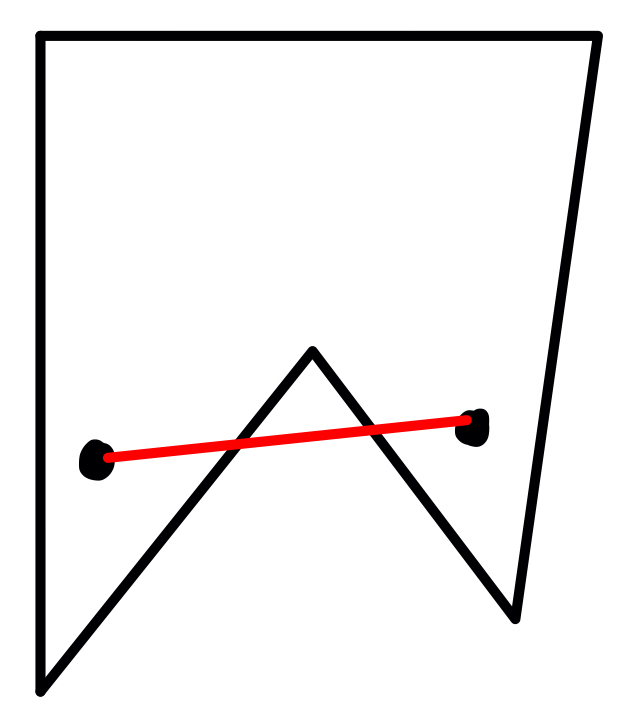
\includegraphics[width=.4\linewidth]{figures/convex-hull-false}
  \caption{Non convex set}
  \label{fig:convex-1}
\end{subfigure}%
\begin{subfigure}{.5\textwidth}
  \centering
  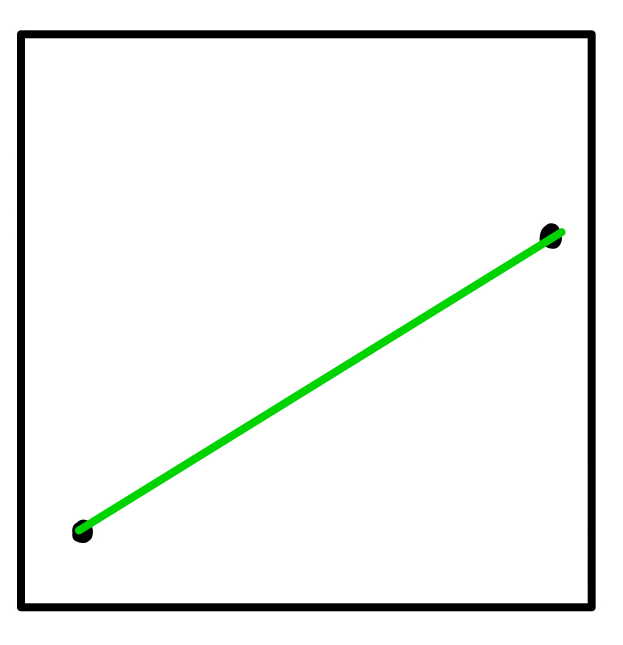
\includegraphics[width=.4\linewidth]{figures/convex-hull-true}
  \caption{Convex set}
  \label{fig:sub2}
\end{subfigure}
\caption{Examples of convex sets}
\label{fig:test}
\end{figure}


\begin{definition}
    Given two points $x = (x_1, x_2)$ and $y = (y_1, y_2)$, the
    convex combination of $x$ and $y$ is defined by
    $$
    \lambda x + (1 - \lambda)y
    $$
    for some $\lambda \in [0, 1]$.
\end{definition}

The convex combination is a way of finding all the points that are in
the line segment of $x$ and $y$.

\begin{definition}
    The convex hull of a finite set of points $S$ is the set of all
    points that can be expressed as convex combinations of points in
    $S$.
\end{definition}

A more pictoral way of defining the convex hull is, given
$S = \{ x_1, ..., x_n \}$, to think of each $x_i$ as a nail, and
we take a rubber band that is originally stretched to infinity, and we
let go of the rubber band. The final position of the rubber band is
the convex hull.

\begin{definition}
    (Another definition of convex hull) The convex hull of a set of
    points is the smallest convex set that
    contains the points.
\end{definition}

\begin{lemma}
    A convex hull is a convex polygon (i.e. not interior angle is
    larger than $\pi$).
\end{lemma}


\subsection{Algorithms to Find the Convex Hull}

Let $(x_1, y_1), ..., (x_n, y_n)$ be the inputs. The output for the
algorithm will be the sequence of points in the boundary in counter
clockwise order.

\subsubsection{Naive Way}

We first produce a simple test: Given a line
by two points and a third point, determine which side of the line the
third point lies on. We claim this is sufficient to find the convex
hull.

To implement this test, suppose we have the line joining $(x_1, y_1)$
and $(x_2, y_2)$ and we consider a point $(x_3, y_3)$. Which side is
this
point on? First, we determine the equation of the line, which is

$$
y - y_1 = \frac{y_2 - y_1}{x_2 - x_1}(x - x_1)
$$

Then we plug in $(x_3, y_3)$ and determine whether $y_3 < mx_3 + b$
or $y_3 > mx_3 + b$ to determine which side of the line the point
lies.

Going back to our naive algorithm:

\begin{itemize}
    \item Take the point $p_k$ with the highest $x$-coordinate. We
    know this
    point must be on the convex hull.
    \item Consider $p_k$ with all other points in $S$.
    \item For each pair $(p_k, p_i)$ check if all the other points lie
    on the same
    side of the line segment joining the pair (use the simple test
    above).
    \item When you find one such pair $(p_k, p_j)$, stop looking for
    more, and repeat this process without considering $p_k$ and
    comparing every other point with $p_j$.
\end{itemize}


This naive algorithm takes $O(n^2)$.


\subsubsection{Divide and Conquer Approach}

\begin{definition}
    A point in one convex hull can \emph{see} a point in another
    convex hull if the segment joining the two points does not
    intersect either hull.
\end{definition}

\begin{definition}
    The upper tangent is the highest line segment joining two points
    on each hull that see each other.
\end{definition}

\begin{definition}
    The lower tangent is the lowest line segment joining two points
    on each hull that see each other.
\end{definition}

\begin{definition}
    We say the line joining point $p$ in hull $C_1$ and point $q$ in
    hull $C_2$ stabs $C_2$ if the continuation of the line goes
    through the interior of $C_2$.
\end{definition}

\begin{remark}
    Recall the simple test above. We can find out when a line stabs
    $C_2$ if the successor of point
    $q$ in $C_2$ is one side of the line and the predecessor of $q$ is
    on the other side of the line.
\end{remark}

The approach for the algorithm is the following:

\begin{itemize}
    \item Divide: Order all points $p_i$ by their $x$-coordinate and
    take the median. Call this point $p_m$. This separates the points
    into two sets, $L$ and $H$.
    \item Conquer: Find the convex hull of $L$ and $H$. The base case
    is when you have three points, which is simply a triangle.
    \item Combine: (Not rigorous at all, mostly shown by picture in
    class) Start by choosing $p$ to be the right-most point in
    the left hull, and $q$ the left-most point in the right hull. Then
    $p$ and $q$ see each other. While the line segment joining these
    two points stabs either $C_1$ or $C_2$, keep "swiveling" these
    until the line segment doesn't stab either hull. You've found the
    upper tangent and lower tangent. This operation takes at most $n$
    for each tangent. Once you've found the upper and lower tangent,
    combine the two hulls as in Figure~\ref{fig:convex-merge}.
\end{itemize}

\begin{figure}[hpt]
    \centering
    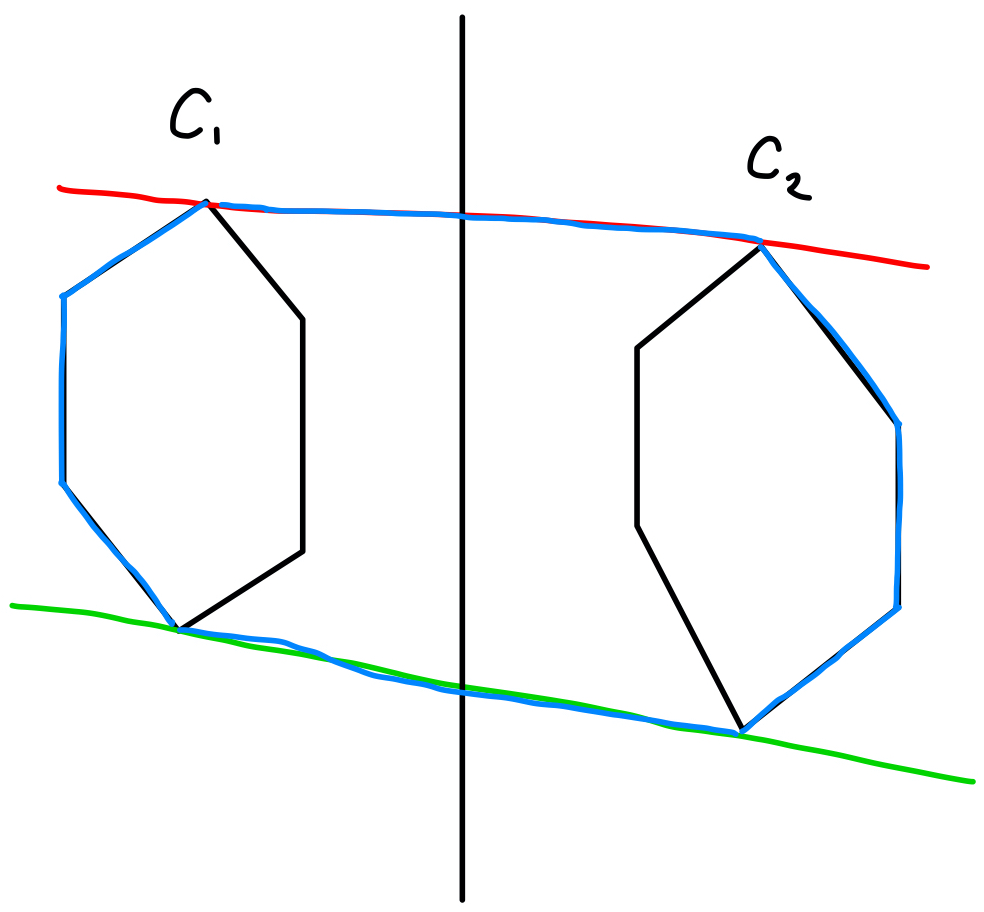
\includegraphics[width=0.4\textwidth]{figures/convex-merge.jpeg}
    \caption{Convex hull combine: In red the upper tangent, in green
    the lower tangent, and in blue the new, merged hull.}
    \label{fig:convex-merge}
\end{figure}








\chapter{Lecture}
%!TEX root = ../main.tex

\section{More Convex Hull}

Convex hulls have many domains. One such examples is in collision detection.

\subsection{Quickhull}

(Spent 5 minutes in class, not very important).
The idea is to get the
point with the minimum $x$-coordinate and the
point
with the maximum $x$-coordinate. Draw a line between these two points,
and hopefully we have divided the points into two sets. Repeat this
for subproblems and merge.

\section{Graphs}

Let $G = (V, E)$ where $V$ is a finite set of vertices and $E$ is a
set of unordered pairs of vertices. There are two representations of
graphs: adjacency lists and adjacency matrices. 

\begin{definition}
    An adjacency list is an array of size $|V|$ where entry $i$ is a
    linked list consisting of the neighbors of vertex $i$.
\end{definition}

\begin{definition}
    An adjacency matrix is a $|V| \times |V|$ matrix $M$ where
    $M_{ij} = 1$ if $(i, j) \in E$ and 0 otherwise. Note the adjacency
    matrix is symmetric for undirected graphs.
\end{definition}

The default representation of graphs is adjacency lists. Note we will
not need to say every time that $G$ is undirected, this
is
implied.

\begin{definition}
    An edge $(u, v)$ has endpoints $u$ and $v$ or equivalently, is
    incident on
    vertices $u$ and $v$. We also say $u$ and $v$ are adjacent if $
    (u, v) \in E$.
\end{definition}

\begin{definition}
    The degree of a vertex $v$ is the number of edges incident on $v$,
    denoted as $d(v) \in \mathbb{N}$.
\end{definition}

\begin{definition}
    A path in a graph $G$ is a sequence of vertices $v_1, v_2, ...,
    v_k$ such that $(v_i, v_{i+1}) \in E$ for all $i = 1 \to k - 1$.
\end{definition}

\begin{definition}
    A path is simple if it does not repeat vertices.
\end{definition}

\begin{definition}
    A (simple) cycle is a sequence of vertices $v_1, v_2, ...,
    v_k$ such that $(v_i, v_{i+1}) \in E$ for all $i = 1 \to k -
    1$ and $(v_k, v_1) \in E$ with the $v_i$ distinct except $v_1$.
\end{definition}

\begin{definition}
    A graph is acyclic if there are no cycles.
\end{definition}

\begin{definition}
    We say $u$ and $v$ are connected if there is a path between them.
    $G$ is connected if for all $u, v \in V$ there is a path
    connecting $u$ and $v$.
\end{definition}

\begin{definition}
    The connected components of $G$ are the maximal subsets of $G$
    that are pairwise connected.
\end{definition}

\begin{remark}
    Connectedness is an equivalence relation.
\end{remark}

\subsection{Trees}

\begin{definition}
    A tree is a connected, acyclic graph.
\end{definition}

\begin{definition}
    (Inductive definition) A rooted tree is either
    \begin{itemize}
        \item A graph consisting of a single vertex $v$ with $v$ as
        the root.
        \item If $(T_1, r_1), (T_2, r_2), ..., (T_k, r_k)$ are rooted
        trees, then the tree $(T, r)$ consisting of a new node $r$ as
        the root and edges $(r, r_1), ..., (r, r_k)$ is a rooted tree.
    \end{itemize}
\end{definition}

Typically problems in this domain can be solved with structural
induction. An example of structural induction is the following:

\begin{lemma}
    Any tree of $n$ nodes has $n - 1$ edges.
\end{lemma}

\begin{proof}
    We prove that any rooted tree on $n$ nodes has $n - 1$ edges which
    implies our lemma. To prove this we first prove the base case.
    Indeed, the statement holds for any single node rooted tree with
    no edges. For the inductive step, we want to prove this for a
    rooted tree built up from $(T_1, r_1), (T_2, r_2), ..., (T_k,
    r_k)$. Assume the statement is true for all the trees $T_i$.
    Tree $T_i$ has $n_i$ nodes. So then $T$ has $1 + \sum_i^k n_i$
    nodes. By the inductive assumption, there are $n_i - 1$ edges in
    $T_i$, so the total number of edges in $T$ is 
    $k + \sum_i^k (n_i - 1) = \sum_i^k n_i$ which is one less than the
    number of nodes, proving our lemma.
\end{proof}

\subsection{Traversals}

How can we traverse a rooted tree? In other words, how can we visit
all the nodes of a tree? We introduce post order traversal.

\begin{algorithm}
\caption{Post order traversal}
\begin{algorithmic}
\REQUIRE{$T$ is a tree with root $r$}
\FOR{child $c$ of $r$}
\STATE{Post order traversal of sub tree with root $c$}
\ENDFOR
\STATE{Visit $r$}
\end{algorithmic}
\end{algorithm}


















\chapter{Lecture}
%!TEX root = ../main.tex

\section{More Graph Traversals}

We continue talking about graph traversals.

\subsection{Breadth First Search (BFS)}

Let $G = (V, E)$ be a graph and let $s \in V$ be the source. The goal of this
algorithm is to visit all the vertices in the graph. A way to visualize BFS is 
picturing a ripple in the water. At time $t$ the algorithm will visit
nodes a distance $t$ from $s$.

There will three possible states for each vertex. 

\begin{itemize}
    \item Undiscovered: A vertex has not yet been visited.
    \item Discovered: Just visited a vertex but not its neighbors.
    \item Finished: Visited vertex and neighbors.
\end{itemize}

\begin{algorithm}
\caption{Breadth first search}
\begin{algorithmic}
\REQUIRE{$G$ a graph,  $s$ a source vertex}
\STATE{$Q = queue(\{s\})$}
\STATE{$seen = \{ s \}$}
\WHILE{$Q$ is not empty}
\STATE{$v = Q.dequeue()$}
\STATE{visit $v$}
\IF{$v$ not in $seen$}
\STATE{$seen = seen \cup \{v\}$}
\FOR{neighbor $n$ in $v$}
\STATE{$Q = Q \cup \{n\}$}
\ENDFOR
\ENDIF
\ENDWHILE
\end{algorithmic}
\end{algorithm}

We can associate levels with the vertices in BFS. The level of $s$ is
0, the neighbors of $s$ have level 1, and so on. Vertex $v$ is
discovered when we dequeue some vertex $u$, and we will set the level
$l
(v) = l(u) + 1$.

\begin{theorem}
    The level of a vertex $v$ is the smallest number of hops to
get from the source $s$ to $v$.
\end{theorem}

\begin{proof}
    Let $\delta(s, v)$ be the smallest number of hops to get from $s$
    to $v$.
    \begin{itemize}
        \item Claim 1: $\delta(s, v) \leq l(v)$. If $v$ has level $l$,
        then there is a sequence of vertices $s, v_1, ..., v_{l-1}, v$
        with $l(v_1) = 1$, $l(v_2) = 2$, and so on. Each vertex was
        discovered from the previous in the sequence. This constitutes
        a path from $s$ to $v$. The smallest path, $\delta(s, v)$,
        must be therefore smaller or equal to this path.
        \item Claim 2: $\delta(s, v) \geq l(v)$. Suppose for a
        contradiction this claim does not hold. For all the $v$ such
        that
        $\delta(s, v) < l(v)$ find the one with smallest $\delta(s,
        v)$. By definition of $\delta$, there is a path from $s$ to
        $v$ with $\delta(s, v)$ hops. Let $s, ..., u, v$ be the path
        with the fewest hops from $s$ to $v$. What does $u$ look like?
        We know $\delta(s, u) = \delta(s, v) - 1$. By the way we
        constructed
        $v$ as being the smallest that contradicts Claim 2, then $u$
        satisfies Claim 2, so therefore $l(u) \leq
        \delta(s, u) = \delta(s, v) - 1$.
        We also know that $l(v) \leq l(u) + 1$. Putting it all
        together, we have that
        $$
        l(v) \leq l(u) + 1 \leq \delta(s, v)
        $$
        which is a contradiction.
    \end{itemize}
\end{proof}

\begin{remark}
    Look at the edges for which new vertices are discovered. These 
edges form a tree (think of the tree as directed away from $s$).
\end{remark}

\subsection{Depth First Search (DFS)}

The idea is that you explore one path as far as it will go, then
backtrack minimally and repeat. More, formally, look at
Algorithm~\ref{alg:dfs}.


\begin{algorithm}
\caption{Depth first search}
\begin{algorithmic}
\REQUIRE{$G$ a graph,  $s$ a source vertex, $seen$ a set}
\STATE{visit $s$}
\STATE{$seen = seen \cup \{ s \}$}
\FOR{each neighbor $n$ of $s$}
\IF{$n$ not in $seen$}
\STATE{recursively call DFS with source $n$}
\ENDIF
\ENDFOR
\end{algorithmic}
\label{alg:dfs}
\end{algorithm}

As in BFS, there will three possible states for each vertex. In BFS
the order of exploration of vertices is the same as the order of
discovery (first in, first out). In DFS, however, we use a stack (or
the recursion stack), so we do last in first out. In other words, the
last discovered vertex is the one first fully explored.

The DFS tree is formed by the set of edges on which new vertices are
discovered.


\begin{lemma}
    If $(u, v)$ is an edge in the graph that is not in the DFS tree,
    then either $u$ is an ancestor of $v$ or $v$ is an ancestor of
    $u$ in the DFS tree.
\end{lemma}

\begin{proof}
    Proof by picture. Do it as an exercise (hint: assume
    contradiction).
\end{proof}


\begin{definition}
The start time $s(u)$ for vertex $u$ is the time for
which DFS of $u$ is invoked, and the finish time $f(u)$ is the time for
which
DFS of $u$ finishes. The duration is the interval from start time to
finish time.
\end{definition}

Note that for all $u, v$ we can't have that $s(u) < s(v) < f(u) <
f(v)$ by the properties of stacks.

Another claim that is useful for DFS is the following. Let's begin
with a wrong, too strong claim.

\begin{lemma}
    (False lemma!). Suppose $u$ is discovered before $v$ and there is a
    path between $u$ and $v$. Then during DFS, $v$ will become a
    descendant of $u$.
\end{lemma}

Why is this wrong? Let's find a counterexample. Consider Figure~\ref{fig:dfs-wrong-lemma}.

\begin{figure}[hpt]
\centering
    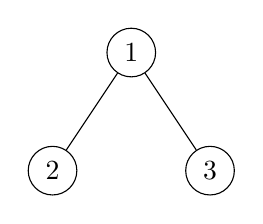
\begin{tikzpicture}[level distance=1.5cm,
                        level 1/.style={sibling distance=2cm}]
  \node[circle, draw=black] {$1$}
    child {node[circle, draw=black] {$2$}} 
    child {node[circle, draw=black] {$3$}};
    \end{tikzpicture}
\caption{Counterexample to the wrong lemma}
\label{fig:dfs-wrong-lemma}
\end{figure}

Suppose DFS visits 2 before 3. There is clearly a path from 2 to 3, 
but 3 is not going to be a descendant of 2. The problem is that the
path between 2 and 3 has vertices that have already been visited.
Let's fix the lemma.

\begin{lemma}
    Suppose $u$ is discovered before $v$ and there is a
    path of undiscovered vertices between $u$ and $v$. Then during
    DFS, $v$ will become a
    descendant of $u$.
\end{lemma}

If you want to prove this, use contradiction.

\section{Connectivity}

\begin{definition}
    A graph is called biconnected if the removal of any vertex leaves
    the graph connected. A graph is called $k$-connected if the
    removal of any $k - 1$ vertices leaves the graph connected.
\end{definition}

A tree is a good example of a connected graph that is not biconnected
(e.g. Figure~\ref{fig:dfs-wrong-lemma}).

\begin{definition}
    A vertex whose removal disconnects the graph is called an
    articulation point.
\end{definition}
 















\chapter{Lecture}
%!TEX root = ../main.tex

\section{More Graphs}

\begin{definition}
    (Informal) Biconnected components are "maximal" pieces of the
    graph that are biconnected.
\end{definition}

Let's define an equivalence relation $R$ on $E \times E$ where
$(e_1, e_2) \in R$ if and only if there exists a simple cycle that
contains $e_1$ and $e_2$ (Exercise: show it's an equivalence
relation). $R$ partitions the edges into equivalence classes $E_1,
..., E_k$. Note that if $R$ only has one equivalence class then the
graph is biconnected. Let component $G_i$ be the graph containing edges in
$E_i$ together with the vertices in $V_i$ consisting of the endpoints
of $E_i$.

Let's go back to DFS. Assume $G$ is connected and start DFS at node
$s$. When is $s$ an articulation point?

\begin{itemize}
    \item Case 1: $s$ has only one child in the DFS tree. In this case
    $s$ is not an articulation point.
    \item Case 2: $s$ has more than one child. Then $s$ is an
    articulation point because non-tree edges go between ancestors and
    descendants. In other words, any vertex in the subtree
    generated by one child of $s$ must
    go through $s$ to reach any vertex in the subtree of another
    child of $s$.
\end{itemize}

What conditions make any vertex $v$ in the DFS tree of $s$ an
articulation point? Suppose $v$ has children $u_1, u_2, ..., u_k$.
An internal node $v$ is an articulation point if and only if
it has a child $u_i$ such that there is no back edge from the subtree
rooted at $u_i$ to a proper ancestor of $v$. See Figure~\ref{fig:articulation} for a diagram.

\begin{figure}
    \centering
    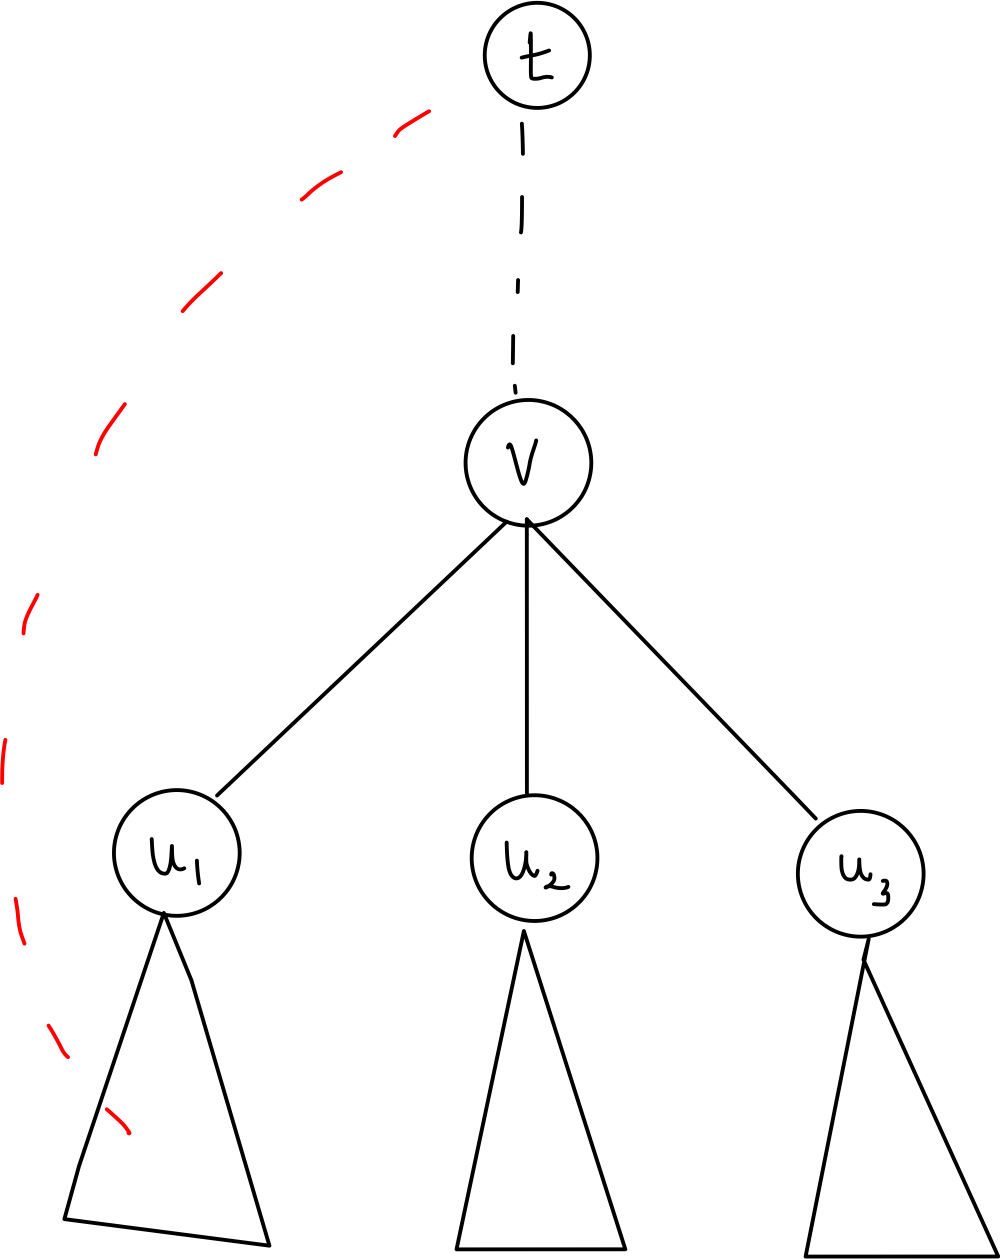
\includegraphics[width=0.3\textwidth]{figures/articulation.jpeg}
    \caption{Condition that makes $v$ an articulation point. In this
    case, it is because the subtree generated by a child of $v$ has a
    back edge to an ancestor of $v$.}
    \label{fig:articulation}
\end{figure}

\subsection{Finding Biconnected Components}

We first must do a DFS starting on a source $s$ and we must do a post
order traversal of the DFS tree as it is produced. As it finds
biconnected components, it outputs them.

Recall that if $u$ is an ancestor of $v$ in the DFS tree, then the
start times $s(u) < s(v)$. Define $\text{low}(x)$ as 
the smallest number (start time) vertex reachable by a back edge from
the subtree rooted at $x$. Suppose for simplicity $v$ has only two
children $u_1, u_2$. Then 

$$
\text{low}(v) = \min(\text{low}(u_1), \; \text{low}(u_2),
\; \underbrace{s(u) : \text{$(v, u)$ is a back edge}}_{\text{we must
consider the back edges of $v$}})
$$

\begin{lemma}
    An internal node $v$ is articulation point if and only if there
    is a child $u_i$ of $v$ such that $\text{low}(u_i) \geq s(v)$.
\end{lemma}

\section{Directed Graphs}

In directed graphs, edges are ordered pairs, so that $(u, v) \in E$
means $u$ is directed to $v$. Naturally, algorithms that we talked
about for undirected graphs might change for directed graphs. Consider
DFS for a directed graph. What type of edges do you encounter? You can
have forward edges, back edges or cross edges. An example of a cross
edge can be seen in Figure~\ref{fig:cross-edge}.

\begin{figure}[hpt]
    \centering
    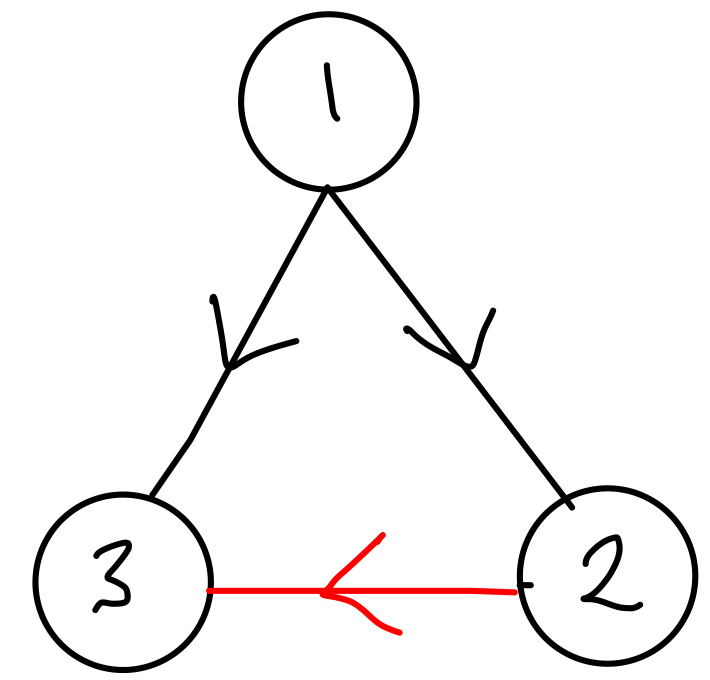
\includegraphics[width=0.2\textwidth]{figures/cross-edge.jpeg}
    \caption{Example of a cross edge in red.}
    \label{fig:cross-edge}
\end{figure}

If $(u, v)$ is a cross edge, then $s(u) > s(v)$.

\subsection{Directed Acylic Graphs (DAGs)}

An example of a DAG is your university course dependency graph, where
some nodes have precedence over others. In general, our goal is to
find an ordering of the vertices such that for each edge $(u, v)$
we have that $u$ precedes $v$ in the ordering. This problem is called
\textbf{topological sorting}.

\begin{lemma}
    Any DAG has a topological ordering.
\end{lemma}

\begin{proof}
    Exercise. Use induction. Or contradiction.
\end{proof}

\begin{definition}
    The in degree of a vertex is the number of incoming edges.
\end{definition}

\begin{theorem}
    If $G$ is a DAG and $(u, v)$ is an edge then for any DFS,
    $f(u) > f(v)$.
\end{theorem}

\begin{proof}

    We show $f(u) > f(v)$.
    \begin{itemize}
    \item Case 1: $s(u) < s(v)$. Then $v$ will become a descendant of
    $u$ (not necessarily a child), so then $f(u) > f(v)$.
    \item Case 2: $s(u) > s(v)$. If we discovered $u$ in the course
    of DFS of $v$, then there must be a path from $v$ to $u$, which
    means $G$ has a cycle, and this is a contradiction. Therefore, 
    $s(v) < f(v) < s(u) < f(u)$
\end{itemize}
In both cases, $f(u) > f(v)$.
\end{proof}

\begin{remark}
    Once you prove this theorem, finding a topological sort of a DAG is
very easy. Find the finish time of all the vertices and output them
in reverse finish time order.
\end{remark}
















\chapter{Lecture}
%!TEX root = ../main.tex

\section{Strongly Connected Components}

Suppose $G = (V, E)$ is a directed graph. What is the correct connectivity
relation in a directed graph? Define a relation $R = \{ (u, v) :
\text{there is a path from $u$ to $v$ and from $v$ to $u$} \}$. Note
we bake into the definition symmetry. For instance, for the graph
$1 \to 2$, we have that $R = \{ (1, 1), (2, 2) \}$. This relation is
in fact an equivalence relation (exercise: show it). We know then
that $R$ partitions $V$ into equivalence classes $V_1, V_2, ..., V_k$.

\begin{definition}
    For any $i = 1 \to k$, we have that 
    $G_i = (V_i, E \cap V_i \times V_i)$ is a strongly 
    connected component of $G$.
\end{definition}

Note that you
could have an edge connecting $G_i$ and $G_j$. Let each $G_i$ denote a
vertex in a new graph $G_{SCC}$. This is the
strongly connected component graph of $G$. More formally,
we have that $G_{SCC} = (V_{SCC}, E_{SCC})$ where 
$V_{SCC} = \{ C_i : C_i \text{is a strongly connected component} \}$
and $E_{SCC} = \{ (c_i, c_j) : \text{there exists
$v_i \in C_i$ and $v_j \in C_j$ such that $(v_i, v_j) \in E$} \}$. For
an example, take a look at Figure~\ref{fig:scc}.

\begin{figure}[hpt]
    \centering
    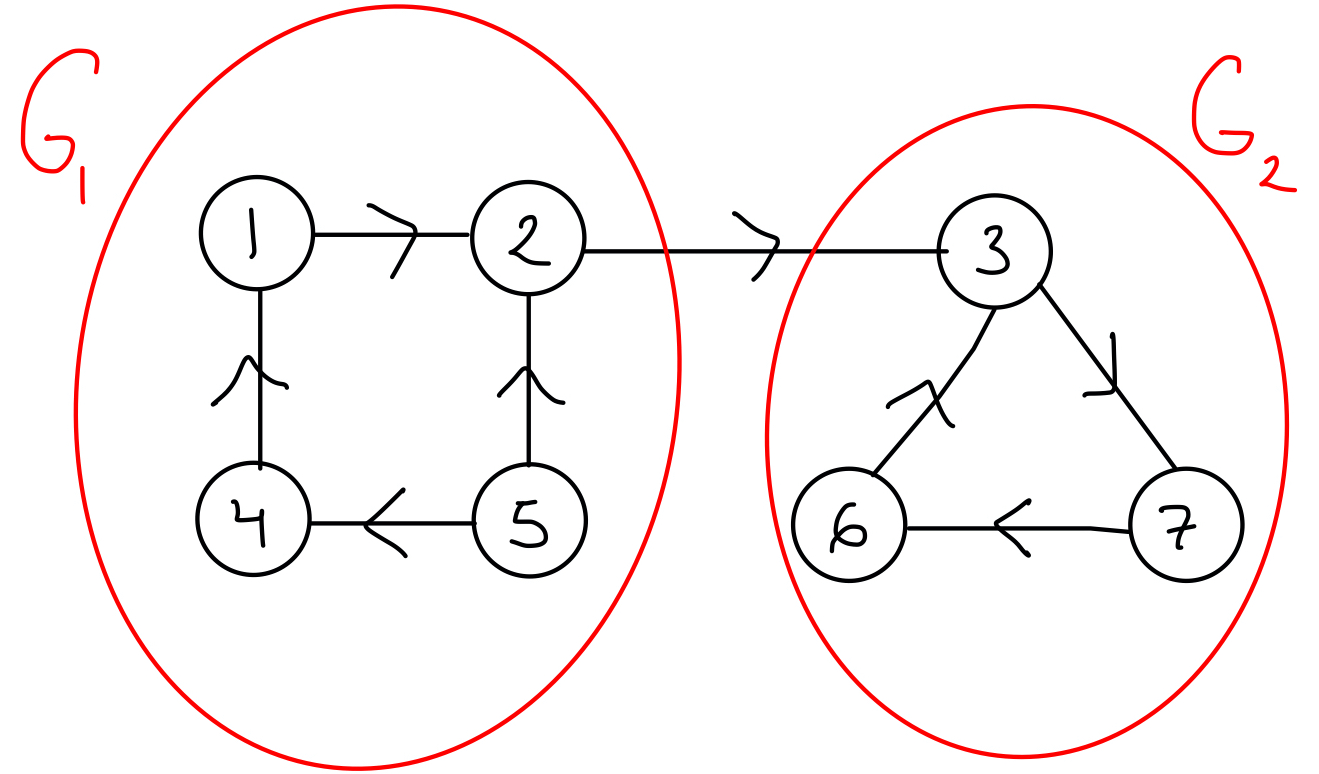
\includegraphics[width=0.45\textwidth]{figures/scc.jpeg}
    \caption{Example of a graph with strongly connected components.
    The
    equivalence classes are $\{\{1, 2, 4, 5 \},  \{3, 6, 7\}\}$. The
    $G_{SCC}$ is simply $C_1 \to C_2$.}
    \label{fig:scc}
\end{figure}

\begin{lemma}
    $G_{SCC}$ is acyclic.
\end{lemma}

DFS will decompose a directed graph $G$ into its SCC. Let $G$ be an
arbitrary directed graph. We know $G_{SCC}$ is a DAG by the above
lemma.

\begin{lemma}
    (False lemma!) If $C_1$ and $C_2$ are SCC and $(C_1, C_2) \in E_
    {SCC}$ then
    in a DFS of $G$, every vertex in $G_1$ finishes after every vertex
    in $G_2$.
\end{lemma}

Why is this wrong? Look at Figure~\ref{fig:scc} and figure it out.

\begin{lemma}
    (Correct lemma) If $C_1$ and $C_2$ are SCC and $(C_1, C_2) \in E_
    {SCC}$ then
    in a DFS of $G$, there exists a vertex in $G_1$ that finishes
    after every vertex
    in $G_2$.
\end{lemma}

\begin{proof}
    Look at the book.
\end{proof}

Let's recapitulate.

\begin{itemize}
    \item We know $G_{SCC}$ is a DAG.
    \item $G_{SCC}$ has one or more vertices with no incoming edges.
    These vertices are called sources. Therefore, if $v$ has the
    largest finishing time $f(v)$ in a DFS of $G$, then $v$ must lie
    in a source component.
\end{itemize}

\subsubsection{Kosaraju's Algorithm}

(Very informal, for more info visit 
\href{https://en.wikipedia.org/wiki/Kosaraju%27s_algorithm}{here}). Perform one DFS to record the
order of finishing times. Let $f_1(v)$ be the finish time of $v$ in this DFS.
Now reverse all the edges in $G$ to create the graph $G^R$ and perform a second DFS of $G^R$ with one constraint: In the outer procedure always choose the undiscovered vertex $v$ with greatest $f_1(v)$ (note that the vertex $v$ with greatest $f_1(v)$ lies in a sink component in $G^R$).
We know $G$ and $G^R$ have the same strongly connected components. We also
know that, since $v$ is in a sink component, the DFS of $G^R$ started at $v$
will only discover the SCC containing $v$. When the inner call to 
DFS($G^R, v$) finishes, output all the discovered vertices as one SCC of $G$.
When we return to the outer loop and pick the undiscovered vertex with
greatest finish time, we know inductively that we will find all SCCs.
The running time of the algorithm is the time it takes to performs two
DFS, which is $O(n)$.

\section{Optimization}

In this type of problems, we would like to minimize/maximize some
function subject to some constraints. A special class of optimizations
problems is the following: Given a set of elements, pick a subset,
where the constraints tell you which subsets are allowed (we call
them \textbf{feasible} solutions). We will have an objective
function that assigns a value to every feasible solution.

\subsection{Minimum Spanning Tree}

The input to this problem is an undirected, connected graph $G = (V,
E)$ together with weights on the edges, where $w: E \to \mathbb{R}^+$.
A feasible solution will be a set of edges that form an acyclic,
connected graph on all vertices. The cost of a solution is the sum of
the weights of the edges in the solution.

\section{Greedy Algorithms}

There are problems for which
the optimum solution can be chosen by choosing one element at a time.
We can solve this problems with greedy algorithms.

\begin{definition}
    A greedy algorithm builds up a solution $S$ by taking at each
    turn the next element with optimal cost that can be added
    feasibly.
\end{definition}

\subsection{Activity Selection Problem}

This is a classic problem that can be solved using a greedy algorithm.
The input is $n$ activities, where $a_i = (s_i, f_i)$ starts at time
$s_i$ and finishes at time $f_i$. A feasible solution will be any
subset of these activities such that no two activities overlap. The
optimization problem will be to maximize the number of activities
scheduled.

Let's propose some criteria to be greedy on.

\begin{itemize}
    \item Pick the activity with shortest duration. This won't work,
    because if you have long activities $n_1 = (1, 10)$ and $n_2 = 
    (11,
    20)$ and a short activity $n_3 = (9, 12)$, this approach will
    only pick $n_3$ with a value of 1 while an optimal solution will
    have a value of 2 (by choosing $n_1$ and $n_2$).
    \item  Pick the activity that finishes first. Sort the activities
    by finish time and reorder them as $a_1, a_2, ..., a_n$ so that
    $f_1 \leq f_2, ... \leq f_n$. Now pick $a_1$ and remove all
    activities that have a conflict with $a_1$, and repeat this
    process.
\end{itemize}

The second approach is correct, but can we prove this? 

\begin{definition}
    The greedy choice property states that the
first choice made by a greedy algorithm is not wrong.
\end{definition}

In this case, the greedy choice property means that if we
choose $a_1$ first, then there is an optimal
feasible solution that contains $a_1$. Suppose for a contradiction
that no optimal solution uses $a_1$. Let $O$ be the subset of
activities in some optimal solution. We can order the activities in
$O$ by finish time. Let $a_{i_1}, ..., a_{i_k}$ be this ordering.
We claim that we can throw away $a_{i_1}$ and replace it with $a_1$.
This is called the \textbf{exchange} argument. We now have $O' = O -
\{a_{i_1}\} \cup \{a_1\}$. But by our greedy assumption the finish
time of $a_1$ is less than the finish time of $a_{i_1}$, so $a_1$
doesn't overlap with $a_{i_2}$ and $O'$ is an optimal solution, which
is a contradiction.

We've just shown there is an optimal solution that starts with $a_1$.
This optimal solution should certainly exclude activities that have a
conflict with $a_1$. Recursively, we need to solve a smaller problem
consisting of activities that don't conflict with $a_1$. In this set
of activities, we need to pick an optimal, feasible subset. 

Let $A$ be the original set of activities, and let $A'$ be the
remaining set of activities after throwing out $a_1$ and its
conflicting activities. Any solution to $A'$ that gives a value of $k$
can be extended to $A$ with value $k + 1$. This shows that we need the
optimal solution to $A'$.

\begin{remark}
    This may seem obvious to you, but there are some problems where
    you need to find a suboptimal solution in $A'$ to get the optimal
    solution for $A$. It just happens to be that for activity
    selection the optimal solution in $A'$ gives the optimal solution
    in $A$.
\end{remark}

\begin{definition}
    A problem is said to have optimal substructure if an optimal
    solution can be constructed from optimal solutions of its subproblems.
\end{definition}

Inductively assume that the greedy approach solves problems with
fewer than $n$ activities optimally. Then the optimal substructure and
the fact that the greedy approach solves the $n$ activity problem
optimally finishes the proof.

\subsubsection{Complexity}

The complexity of this problem is $O(n\log(n))$, as we need to sort
the activities by finish time.













\chapter{Lecture}
%!TEX root = ../main.tex

\section{Vector Spaces Review}

\begin{definition}
    $V$ is vector space over $\mathbb{R}^n$ if
    \begin{itemize}
        \item For any $v_1, v_2 \in V \implies v_1 + v_2 \in V$.
        \item For any $\alpha \in \mathbb{R}$ and $v \in V$ then
        $\alpha v \in V$.
    \end{itemize}
\end{definition}

\begin{definition}
    Given a finite set of vectors $v_1, ..., v_k$, the span $S(v_1,
    ..., v_k)$ is the set of all linearly combinations, i.e.
    $$
    S(v_1, ..., v_k) = \{\alpha_1v_1 + ... + \alpha_kv_k : \alpha_i
    \in \mathbb{R}\}
    $$
\end{definition}

\begin{definition}
    A set of vectors $v_1, ..., v_k$ is linearly dependent if there
    exist some non-trivial $\alpha_1, ..., \alpha_k$ with
    $$
    \alpha_1v_1 + ... + \alpha_kv_k = 0
    $$
\end{definition}

\begin{lemma}
    The span is a vector space.
\end{lemma}

\begin{definition}
    A set of vectors is said to be linearly independent if they are
    not linearly dependent.
\end{definition}

\begin{definition}
    Let $v_1, ..., v_k$ be linearly independent and suppose their
    span is $V$, then $v_1, ..., v_k$ form a basis for $V$.
\end{definition}

\begin{lemma}
    If $v_1, ..., v_k$ is a basis for $V$ and $u_1, ..., u_k$ is
    another basis for $V$, then $m = k$.
\end{lemma}

\begin{proof}
    (Sketch). Suppose for a contradiction that $m > k$. Then we have
    \begin{align*}
        u_1 &= \alpha_{11}v_1 + ... + \alpha_{1k}v_k \\
        u_2 &= \alpha_{21}v_1 + ... + \alpha_{2k}v_k \\
        \vdots \\
        u_m &= \alpha_{m1}v_1 + ... + \alpha_{mk}v_k
    \end{align*}
    We need to show that $u_1, ..., u_m$ is linearly dependent. To
    show this, we need to find some non-trivial $x_1, ..., x_m$ such
    that $\sum_i x_iu_i = 0$. So suppose $\sum_i x_iu_i = 0$.
    Substitute each $u_i$ with the equations above. Collect terms, and
    you'll get a system of equations with $k$ equations and $m$
    unknowns, which leads to infinitely many solutions since $m > k$
    by assumption. This leads to a contradiction.
\end{proof}

\section{More Greedy Algorithms}

\subsection{Basis of Maximal Weight}

Problem: Suppose you are Google and you assign a vector to each
possible
document. When a user searches for a term, you want to collect some
vectors that are indicative of that search term. You also want to be
diverse, e.g., if a user searches for "jaguar" you want to return
some documents with cars and others with the animal. We could model
this by returning vectors that are linearly independent.

More abstractly, given vectors $v_1, ..., v_n$ with weights $w_1, ...,
w_n$, we need to return a basis (note there can be many!) for the
space spanned by these vectors of maximum total weight.

\subsubsection{Greedy Approach}

Sort the vectors by decreasing order of weights $v_1, ..., v_n$. Let
$S$ be a set of vectors. For each vector $v_i$ in this order, if $S
\cup \{v_i\}$ is linearly independent, then assign $S = S \cup 
\{v_i\}$.

\subsubsection{Correctness}

By contradiction. Suppose the greedy approach returns vector $v_{i_1},
..., v_{i_k}$,
and suppose there is an optimal solution that returns vectors
$v_{j_1}, ..., v_{j_k}$. Because the $v_j$ form a basis, $v_{i_1}$ can
be expressed as a linear combination of the $v_j$'s. Indeed,

$$
v_{i_1} = \alpha_1v_{j_1} + ... + \alpha_1v_{j_k} 
$$

Notice some $\alpha_l \neq 0$. We can add $v_{i_1}$ into the set
$v_{j_1}, ..., v_{j_k}$ and throw out $v_{j_l}$. We claim this is also
a basis with weight at least as good.

\chapter{Lecture}
%!TEX root = ../main.tex

(No video recording, looking for notes for this lecture. Have them? Submit a pull request!)

\chapter{Lecture}
%!TEX root = ../main.tex

\section{Kruskal's Algorithm}


Kruskal's algorithm finds a minimum weight spanning tree in a 
connected, weighted, undirected graph. 

\begin{itemize}
    \item Step 1: Sort and renumber the edges in increasing
order of weight as $e_1, ..., e_n$. 
    \item Step 2: Create a graph $G$ with the same vertices as the
    original
    graph.
    \item Step 3: For each edge $e_i = (u, v)$, add the edge
    to the graph if and only if $u$ and $v$ lie in different
    components. To do this, we need two routines.
    \begin{itemize}
        \item Find: return the component for a vertex $u$.
        \item Union: merge two components together.
    \end{itemize}
    We are going to define a \href{https://en.wikipedia.org/wiki/Disjoint-set_data_structure}{union-find} data structure to
    solve this, which we will initialize to $n$ singleton components.
\end{itemize}

\subsubsection{Union-Find}

Let's look at various attempts to implement this data structure.

\begin{enumerate}
    \item First attempt. Keep an array where the index $i$ tells you
    what
    component $v_i$ is in. Initially, each vertex belongs to its
    component, so the array is $A = [1, 2, 3, ..., n]$. We immediately
    notice that we can perform the find operation in
    $O(1)$ (just index into the array). What about union of $u$ and
    $v$? This takes $O(n)$ (you might need to reassign $n - 1$
    components). Using this approach, in
    the course of Kruskal's algorithm we will perform $n - 1$ unions 
    (we start from $n$ components and get to 1 component). Each takes
    order $n$, so we'll get overall $O(n^2)$. We want to do better.
    \item Second attempt. 
    Notice that when we perform union($u, v$), $u$'s set contains
    $n_1$ elements and $v$'s set contains $n_2$ elements. To do less
    operations, we ideally want to change the components of the set
    that is smaller. This operation still takes in the worst case $O
    (n)$. In this attempt, in addition to the array, we maintain a
    linked list for each set containing the elements in that set 
    (think of it as a reverse indexing from the component to the
    elements). An
    individual union operation could still take $\Theta(n)$ steps.
    However, any $k$ union operations performed by Kruskal take only
    $O(k\log(n))$ steps. We've moved from analyzing one operation to
    analyzing a sequence of operations (amortized analysis, we'll
    talk about this in a minute). Indeed, suppose you take the union
    of $A$ and $B$, where $|A| > |B|$. The cost of the operation is
    equal to the size of $B$. Set up a counter for each element in
    the data structure, and charge 1 to each element in $B$ for a
    union operation. How many times does an element get charged? Every
    time an element is charged, it joins a set that is as twice as
    large. Therefore, we can charge at most $\log(n)$ times, so the
    total cost of all $n - 1$ unions is $n\log(n)$. More careful
    analysis will show you that $k$ unions cost at most $k\log(k)$.
    This is an example of amortized analysis.
    \item Third attempt. The idea is to maintain each connected
    component as a tree (see Figure~\ref{fig:kruskal}). How long does
    the find operation
    take? Say
    the name of the component is the element at the root of the tree.
    For each node in the tree, keep a pointer to its parent.
    Finally, traverse up the tree until you find the root and you will
    have found the component. The cost is proportional to the height
    of each tree (note that all tree heights at all
    times are $O(\log(n))$, so this is what it costs to do a find). 
    To do a union operation, have one root point to the
    other root. We can do the same amortized trick we performed above,
    and we can make the root of the tree with fewer elements point up
    to the root of the other tree. Unions of arbitrary pairs of
    elements is also $O(\log(n))$. We've established that Kruskal
    performs $n - 1$ unions, but how many finds does it perform? It
    does $O(m)$ finds. Therefore, performing all the union-finds takes
    $O(m\log(n))$.
\end{enumerate}

\begin{figure}[hpt]
    \centering
    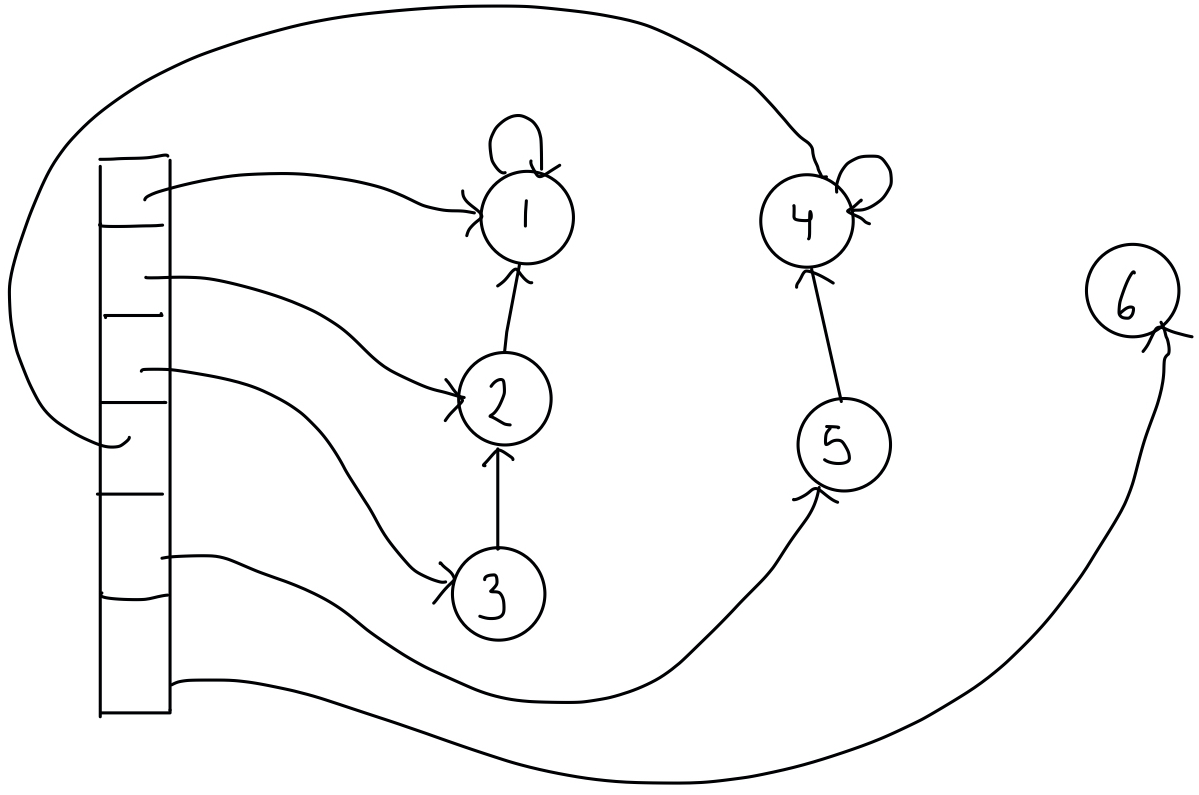
\includegraphics[width=0.65\textwidth]{figures/kruskal.jpeg}
    \caption{Data structure used for the third attempt}
    \label{fig:kruskal}
\end{figure}

The time complexity for Kruskal is $O(m\log(n))$. Indeed, we have to
first sort the edges by weights, so the union-finds are not in fact
the bottleneck. One optimization in the third attempt is called path
compression. The idea is that when you perform find($u$), for each
vertex encountered from the path from $u$ to the root, make it a child
of the root. 

Any sequence of $m$ operations starting from the initial
union find data structure on $n$ elements takes at most $O(m\log^*
(n))$ time, where $\log^*(x)$ is the number of times you need to take
the log of $x$ to make the value less than or equal to 1. For
instance,
$\log^*(16) = 3$, since you need to do $16 \to 4 \to 2 \to 1$.
The fact is $\log^*(n)$ is a \textbf{really} slow growing
function, so we can take interpret it as a constant. For example,
$\log^*(2^{16} = 65,536) = 4$, and $\log^*(2^{65,536}) = 5$. This is
more than the number of particles in the universe, so there's no way
that you will get a problem with an input bigger than this. Therefore,
we can treat it as almost constant.

\subsection{Prim's Algorithm}

In Prim's algorithm, we keep a set $S$, which we call the source side,
and we consider $V - S$, the remaining vertices that are not in $S$.
At every step we take the cheapest edge joining $S$ and
$V - S$. For each $v \in V - S$, maintain $d(v)$, which is the
weight of the cheapest edge from $v$ to some vertex in $S$. 

Initially, $S = \{ s \}$, and for every $v \in V - S$, we have that
$d(v) = w(s, v)$ if $(s, v)$ is an edge and $\infty$ otherwise. At
each iteration (see Figure~\ref{fig:prim}), when we move the vertex
$y$ that has the cheapest edge to a vertex in $S$, we need to update
every neighbor $v$ of $y$ so that $d(v) = \min(d(v), w(v, y))$.

\begin{figure}[hpt]
    \centering
    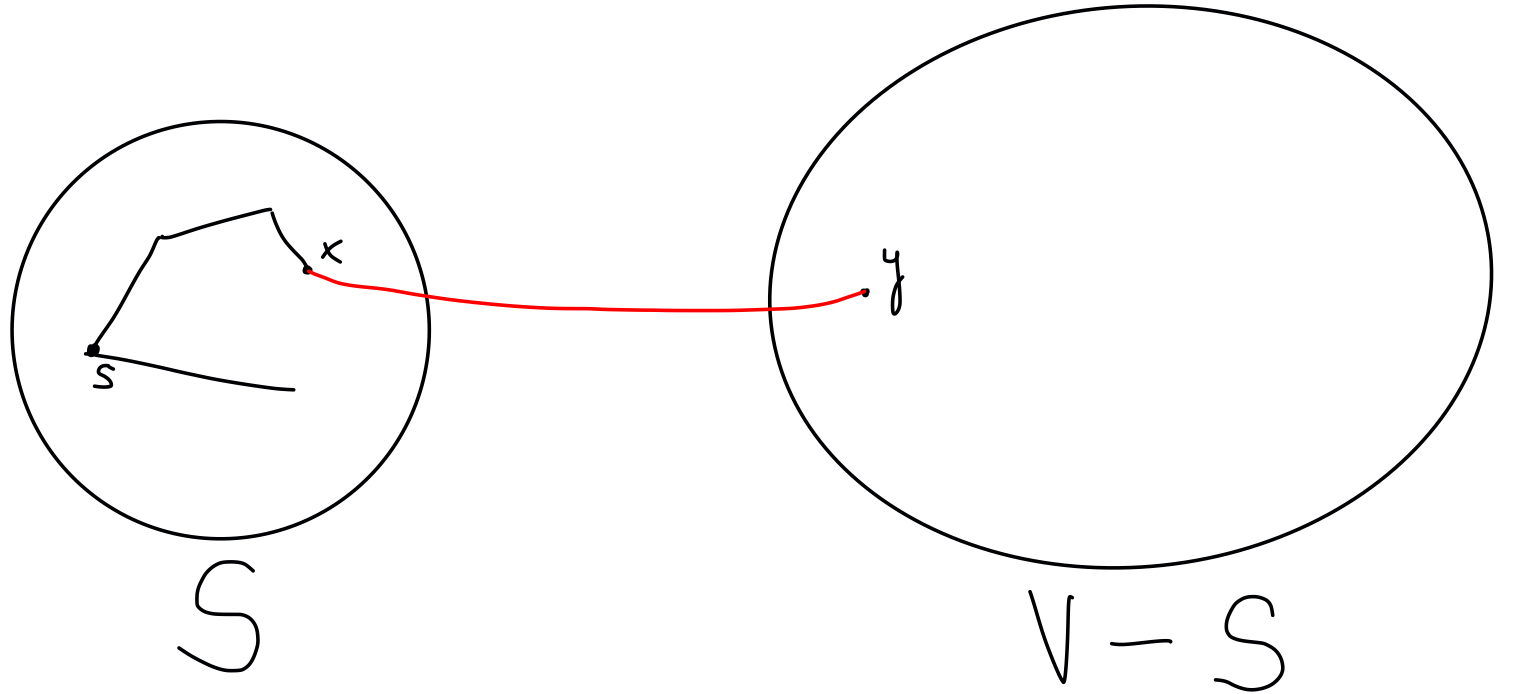
\includegraphics[width=0.65\textwidth]{figures/prim.jpeg}
    \caption{Prim's algorithm visualization}
    \label{fig:prim}
\end{figure}

\subsubsection{Time Complexity}

If we maintain the $d(v)$s in an array $A$, the complexity is $O(n^2)$
because we need to first find the minimum in $A$, and once we've found
the minimum we need to update all the neighbors of the minimum.

If we maintain the $d(v)$s in a min-heap, the complexity is $O(m\log
(n))$.

\section{Shortest Paths}

Let $G = (V, E)$ be a directed, weighted graph with a weight function
$w : E \to \mathbb{R}$. We assume $G$ is directed because we can
easily convert undirected shortest paths to directed shortest paths.

One common variation for this problem is the single source shortest
path. The problem is to find the shortest path from a given vertex $s$
to all the other vertices. Another variant is all-paths shortest path,
in which we need to find the shortest path from any $u$ to any
$v$.

\subsection{Single Source Shortest Path}

We will assume all edge weights are non negative, and we will solve
this using Dijkstra's Algorithm. The idea is to maintain a quantity $d
(v)$ for each vertex $v$ which is an upper bound on the length of the
shortest path from $s$ to $v$.













%\bibliography{bibfile}

\end{document}